
% ------------------------------------------------------------------------
% ------------------------------------------------------------------------
% abnTeX2: Modelo de Trabalho Academico (tese de doutorado, dissertacao de
% mestrado e trabalhos monograficos em geral) em conformidade com 
% ABNT NBR 14724:2011: Informacao e documentacao - Trabalhos academicos -
% Apresentacao
% MODELO DE PROJETO DE PESQUISA - UESPI
% ------------------------------------------------------------------------
% 


\documentclass[
	% -- opções da classe memoir --
	12pt,				% tamanho da fonte
	openright,			% capítulos começam em pág. ímpar (insere página vazia caso preciso)
	oneside,			% para impressão em verso e anverso. Oposto a oneside
	a4paper,			% tamanho do papel. 
	% -- opções da classe abntex2 --
	chapter=TITLE,		% títulos de capítulos convertidos em letras maiúsculas
	%section=TITLE,		% títulos de seções convertidos em letras maiúsculas
	%subsection=TITLE,	% títulos de subseções convertidos em letras maiúsculas
	%subsubsection=TITLE,% títulos de subsubseções convertidos em letras maiúsculas
	% -- opções do pacote babel --
	english,			% idioma adicional para hifenização
	%french,				% idioma adicional para hifenização
	%spanish,			% idioma adicional para hifenização
	brazil,				% o último idioma é o principal do documento
	]{abntex2}
% ---
% Pacotes básicos 
% ---
%\usepackage{lmodern}			% Usa a fonte Latin Modern	
\usepackage{mathptmx}
\renewcommand{\ABNTEXchapterfont}{\normalfont}
%\usepackage{bookman}		
\usepackage[T1]{fontenc}		% Selecao de codigos de fonte.
\usepackage[utf8]{inputenc}		% Codificacao do documento (conversão automática dos acentos)
\usepackage{lastpage}			% Usado pela Ficha catalográfica
\usepackage{indentfirst}		% Indenta o primeiro parágrafo de cada seção.
\usepackage{color}				% Controle das cores
\usepackage{graphicx}			% Inclusão de gráficos
\usepackage{microtype} 			% para melhorias de justificação

\usepackage{subcaption} %subcaptions em subfigures

\usepackage{epigraph}

%Depois no documento escrevemos:

%\epigraph{texto}{referência}


%\usepackage{geometry}
%\geometry{a4paper, left=3cm, right=2cm, bottom=2cm, top=3cm}
% ---
\graphicspath{ {./figs/} }
% ---
% Pacotes adicionais, usados apenas no âmbito do Modelo Canônico do abnteX2
% ---
\usepackage{lipsum}				% para geração de dummy text
% ---
% Pacotes de citações
% ---
\usepackage[brazilian,hyperpageref]{backref}	 % Paginas com as citações na bibl
\usepackage[alf]{abntex2cite}	% Citações padrão ABNT
% Pacotes adicionais ++
\usepackage{listings}

% --- 
% CONFIGURAÇÕES DE PACOTES
% --- 

% ---
% Configurações do pacote backref
% Usado sem a opção hyperpageref de backref
\renewcommand{\backrefpagesname}{Citado na(s) página(s):~}
% Texto padrão antes do número das páginas
\renewcommand{\backref}{}
% Define os textos da citação
\renewcommand*{\backrefalt}[4]{
	\ifcase #1 %
		Nenhuma citação no texto.%
	\or
		Citado na página #2.%
	\else
		Citado #1 vezes nas páginas #2.%
	\fi}%
% ---


%%%%%comandos para revisão
\newcommand{\supervisor}[1]{\textcolor{red}{[#1]}}

\newcommand{\aluno}[1]{\textcolor{blue}{[#1]}}


%================================================================================
% Pacote para criacao da lista de siglas e abreviaturas
%================================================================================
\usepackage{nomencl}
\makeatletter
\setlength{\nomlabelwidth}{0.15\hsize} 
\renewcommand{\nomlabel}[1]{#1 \hfill}
\setlength{\nomitemsep}{-.05in} 
\makenomenclature
% Traduz o titulo da lista de abreviaturas
\renewcommand{\nomname}{Lista de Abreviaturas e Siglas}

% Comando para criacao de abreviaturas e siglas
\def\sigla{\@ifstar\@sigla\@@sigla}
% Apenas faz o registro na tabela de siglas
\def\@sigla#1#2{\nomenclature{#1}{#2}}          % \sigla*{}{} 
% Faz o registro na tabela de siglas e insere os dados no corpo do documento
\def\@@sigla#1#2{#2 (#1)\nomenclature{#1}{#2}}  % \sigla{}{}
\makeatother
%%%%%%%%%%%
%%%Lista de quadros


\usepackage{float}
\floatstyle{plaintop} % Coloca caption no topo
\newfloat{quadro}{htbp}{lop}
\floatname{quadro}{Quadro}
\newcommand{\listofquadros}{\listof{quadro}{Lista de Quadros}}
\def\quadroautorefname{Quadro}
%%%Lista de quadros




% ---
% Informações de dados para CAPA e FOLHA DE ROSTO
% ---
\titulo{Geração de Modelo 3D a partir de Planta Baixa 2D}
\autor{João Pedro Barros do Nascimento}
\local{Teresina}
\data{2025}
\orientador{Carlos Giovanni Nunes de Carvalho}
\instituicao{Universidade Estadual do Piauí}
\tipotrabalho{Projeto de Pesquisa (Graduação)}

% O preambulo deve conter o tipo do trabalho, o objetivo, o nome da instituição e a área de concentração 
\preambulo{Pré-projeto de Trabalho de Conclusão de Curso apresentado na Universidade Estadual do Piauí – UESPI como parte dos requisitos para conclusão do Curso de Bacharelado em Ciência da Computação.}



% Configurações de aparência do PDF final
%\definecolor{blue}{RGB}{41,5,195}
% informações do PDF
\makeatletter
\hypersetup{
     	%pagebackref=true,
		pdftitle={\@title}, 
		pdfauthor={\@author},
    	pdfsubject={\imprimirpreambulo},
	    pdfcreator={LaTeX with abnTeX2},
		pdfkeywords={abnt}{latex}{abntex}{abntex2}{trabalho acadêmico}, 
		colorlinks=true,       		% false: boxed links; true:              colored links
    	linkcolor=black,          	% color of internal links
    	citecolor=black,        		% color of links to bibliography
    	filecolor=magenta,      		% color of file links
		urlcolor=black,
		bookmarksdepth=4}

\makeatother
% --- 
% Espaçamentos entre linhas e parágrafos 
% --- 
% O tamanho do parágrafo é dado por:
\setlength{\parindent}{1.3cm}
% Controle do espaçamento entre um parágrafo e outro:
\setlength{\parskip}{0.2cm}  % tente também \onelineskip
% ---
% compila o indice
% ---
\makeindex
% ---

% --------------------------------------------------------------------------------------------------------
% % Início do documento
% --------------------------------------------------------------------------------------------------------
\begin{document}

% Retira espaço extra obsoleto entre as frases.
\frenchspacing 

%%capa
% Capa
% A capa no projeto de pesquisa é opcional
%---------------------------------------------------------------------------------------------------------

    \begin{center}
    {\ABNTEXchapterfont\large UNIVERSIDADE ESTADUAL DO PIAUÍ}\\
    {\ABNTEXchapterfont\large CIÊNCIA DA COMPUTAÇÃO}
    
    \vspace*{\fill}\vspace*{\fill}
    {\ABNTEXchapterfont\large \imprimirautor}  
    \vspace*{\fill}
   
    \vspace*{\fill}\vspace*{\fill}
    \begin{center}
    \ABNTEXchapterfont \bfseries \Large \imprimirtitulo
    \end{center}
    \vspace*{\fill}\vspace*{\fill}
   
  
   \end{center}  

      
    \begin{center}
    \vspace*{0.5cm}
    {\ABNTEXchapterfont\large TERESINA}
    \par
    {\ABNTEXchapterfont\large \imprimirdata}
    \vspace*{1cm}
    \end{center}
%--------------------------------------------------x------------------------------------------------------

%%



% Folha de Rosto
% --------------------------------------------------------------------------------------------------------
\begin{folhaderosto}

  \begin{center}
    {\ABNTEXchapterfont\large \imprimirautor}

    \vspace*{\fill}\vspace*{\fill}
    \begin{center}
      \ABNTEXchapterfont\bfseries\Large \imprimirtitulo
    \end{center}
    \vspace*{\fill}
    
    \hspace{.45\textwidth}
    \begin{minipage}{.5\textwidth}
        \imprimirpreambulo
    \end{minipage}%
    
    \vspace{1.5cm}
    Orientador: \imprimirorientador \\
    
    \vspace*{\fill}
     
   \end{center}  

     \begin{center}
    \vspace*{0.5cm}
    {\ABNTEXchapterfont\large TERESINA}
    \par
    {\ABNTEXchapterfont\large \imprimirdata}
    \vspace*{1cm}
    \end{center}
  
\end{folhaderosto}
%--------------------------------------------------x----------------------------------------

% Resumo
%---------------------------------------------------------------------------------------------------------
\setlength{\absparsep}{18pt} % ajusta o espaçamento dos parágrafos do resumo
\begin{resumo}
\ABNTEXchapterfont
No seu resumo de projeto de pesquisa você deve em um paragrafo contínuo apresentar, de forma concisa e informativa, o tema, os objetivos da pesquisa, a metodologia a ser utilizada, os principais resultados que espera alcançar, tudo em um parágrafo único e no tempo verbal adequado para cada parte. O resumo deve seguir a NBR 6028 da \sigla{ABNT}{Associacao Brasileira de Normas Tecnicas}, ser escrito em terceira pessoa, sem recuos na primeira linha, e ser acompanhado de palavras-chave que representem o conteúdo da monografia. 

\textbf{Palavras-chaves}: Planta baixa; Geração 3D; 3D .
\end{resumo}
%--------------------------------------------------x------------------------------------------------------


% Abstract
%---------------------------------------------------------------------------------------------------------
\begin{resumo}[Abstract]
\ABNTEXchapterfont
In the Computer Science course, introductory subjects play a crucial role in the development of student knowledge, expanding their theoretical base and enhancing essential skills for problem-solving. Among these skills, data analysis, manipulation, and treatment stand out, which are acquired through the Database subject and are fundamental for obtaining and processing information. Despite the proven importance of Database concepts, it is noted that students face challenges, such as demotivation resulting from the exhausProtive learning process, which can affect focus, proactivity, and the acquisition of necessary knowledge. Given these challenges, it becomes essential to adopt alternative teaching approaches that can mitigate the students theoretical deficiencies. Gamification, which incorporates game design elements in non-playful environments, can be used to increase student engagement, encouraging them to perform tasks and achieve pre-established objectives. In this context, the main objective of this project is to develop a framework that defines design metrics based on gamification elements, aiming at the effective construction of gamified teaching applications focused on teaching the concepts of Relational Database and SQL language.

% \begin{otherlanguage*}{english}
%   This is the english abstract.
%   \vspace{\onelineskip}
%   \noindent 

\textbf{Keywords}: Gamification; Relational Database; Teaching Framework.
\end{resumo}
%--------------------------------------------------x------------------------------------------------------


% inserir lista de ilustrações
%---------------------------------------------------------------------------------------------------------
\pdfbookmark[0]{\listfigurename}{lof}
\listoffigures*
\cleardoublepage
%--------------------------------------------------x------------------------------------------------------


% inserir lista de tabelas
%---------------------------------------------------------------------------------------------------------
% \pdfbookmark[0]{\listtablename}{lot}
% \listoftables*
% \cleardoublepage
%--------------------------------------------------x------------------------------------------------------


% inserir lista de abreviaturas e siglas
%-------------------------------------------------------------------------------------------
% para inserir as  abreviaturas e siglas use no texto o comando \sigla{SIGLA}{DEFINICAO DA SIGLA}a primeira vez que for definir a sigla 
%---------------------------------------------------------------------------------------------------------
\printnomenclature
\cleardoublepage
%--------------------------------------------------x------------------------------------------------------

%%%Lista de codigos
% Inclui a lista de códigos
%\incluilistadecodigos



%%Lista de quadros
\pdfbookmark[0]{\listtablename}{lot}
\listofquadros
\cleardoublepage

%--------------------------------------------------x------------------------------------------------------
\pdfbookmark[0]{\contentsname}{toc}
\tableofcontents*
\cleardoublepage
\textual
%--------------------------------------------------x------------------------------------------------------
                                          % INTRODUÇÃO %
%---------------------------------------------------------------------------------------------------------
\chapter{Introdução}\label{cp:introducao}
\ABNTEXchapterfont

% Contextualização problema em questão
% O que encontrei na bibliografia

% % Motivação do avanço tecnologico que motivou a utilização dessa técnica ao ínves das anteriores

% 2021Alibaba: Capítulo 2,¶1 e ¶2 :
% [...] Traditional methods [8, 9, 10] focus on directly processing low-level features. These systems produce a large number of hand-designed features and models. [...] Those systems mentioned above bring the problem of insufficient generalization ability. Thresholds and features are adjusted frequently by handcrafted operations instead of automatic methods. 
% With the development of deep learning techniques, the method of obtaining room structure has made significant process in generalization. Convolutional Neural Network (CNN) can create and extract advanced features to enhance the recognition performance of room elements [22, 29, 33]. Liu et al. [22] illustrate junctions of floor plans, for example, corners of walls, could be recognized by CNN [...]. However, the approach has limitations, for instance, it is not able to detect inclined walls. [...]. 

% - Justificativa digitalização dos documentos e utilização de
% dados quantitativos(monetário) na justificativo ( a lá redação enem )
% Dados quantitativos 
% MultiFloor: "Urban areas experience a steady growth, and over two-thirds of the population worldwide will be considered urbanized by the year 2050[1]" -> https://population.un.org/wup/assets/WUP2018-Report.pdf % Pegar a versão atualizada desse texto

% Dados qualitativos 
% MultiFloor: "may benefit multiple fields and subdomains, such as creating virtual twins of buildings [2], optimal evacuation path planning [7], and firefighting " 
% 2021Alibaba: "after the above rasterization process, designers cannot modify the structure of the room and redesign flexibly. Therefore, accurately recovering vectorized information from pixel images becomes an urgent problem to be solved."
% Precisa de uma referência que cita projetos de renovação

% Dados que justificam o uso da planta 3D ao invés da 2D
% ex: diminuição de custo, segurança pública

% Escrita
% Premissa: Há uma necessidade de utilizar gerar modelos 3D a partir de plantas 2D
A recuperação do modelo arquitetônico,\sigla{BIM}{Building Informational Model}, a partir de um planta baixa é uma necessidade que arquitetos e designers precisam para modificar e alterar o projeto \cite{lv2021residential}, pois todos os projetos atuais \iffalse achismo sem referencia \fi são feitos com um auxilio do computador.
Além disso, há a necessidade da criação do modelo 3D para planejar rotas de fuga e combate a incêndios \cite{kratochvila2024multi}.


\section{Objetivos}\label{cp:intro:obj}
Considerando a contextualização apresentada, nessa seção temos os objetivos gerais e específicos desse projeto de pesquisa.

\subsection{Objetivo Geral}\label{cp:intro:objgeral}
Desenvolver uma programa para gerar uma modelo 3D através de uma imagem de uma planta baixa de acordo com técnicas de processamento de imagem e detecção de característica. % das quais utilizando técnicas de baixo custo de hardware\cite{yang2022automated}.

\subsection{Objetivos Específicos}\label{cp:intro:objespec}
\begin{itemize}
  \item Revisão bibliográfica melhor entender as técnicas das referências, já que não está disponível o código fonte e com base na revisão recriar a arquitetura.
  \item Treinar o modelo de acordo com a literatura e os datasets. % Datasets como o CubiCasa5K.
  \item Coletar das plantas baixas para serem processadas. % Digitalizar as plantas baixas disponíveis de Teresina.
  \item Gerar modelos 3D a partir das plantas baixas. % Executar o modelo e exportar para um formato de arquivo 3D: $.obj$ ou $.gltf$
  \item Exibir o modelo 3D gerado.%  Utilizando o framework ThreeJS \iffalse baseado em qual artigo que a escolhar do ThreeJS é valida? os artigos utilizam alguma forma de exibição mas não disseram qual e como especificamente \fi exibindo o desenho 3D, no navegador com o controle de órbita e $panning$.
\end{itemize}


\section{Organização do Trabalho}\label{cp:intro:organization}
Esta monografia está estruturada em 4 capítulos. O \autoref{cp:introducao} tem como objetivo mostrar ao leitor um panorama geral do trabalho, incluindo a contextualização ao qual a pesquisa está inserida, a justificativa e os objetivos geral e específicos. O \autoref{cp:refteory} apresenta o referencial teórico necessário para fundamentar os principais conceitos diretamente relacionados com a pesquisa a ser desenvolvida. No \autoref{cp:revisaoliteraria} são apresentados o protocolo de revisão literária, tal como os trabalhos relacionados com a proposta dessa pesquisa. No \autoref{cp:metodologia} são apresentados a classificação da pesquisa, o método a ser aplicado, o cronograma de desenvolvimento da monografia assim como os resultados que se espera alcançar através desta pesquisa. 

O trabalho é finalizado com a apresentação das referências bibliográficas que estruturaram a apresentação dos conceitos que constituem este estudo.






%--------------------------------------------------x------------------------------------------------------
\chapter{Referencial Teórico}\label{cp:refteory}
\ABNTEXchapterfont
% Justificativa das tecnologias, comparação 
%Este capítulo é um componente importante para esse estudo, pois fornece uma base  explorando as principais teorias, conceitos e definições existentes sobre as áreas de conhecimento que motivaram a elaboração deste projeto de pesquisa e que guiarão a execução do percurso metodológico.

%Escreva sobre o referencial teórico do seu trabalho

% Qual é o tipo de problema
% Utilizando o artigo do 3DPlanNet
O desenho arquitetônico descreve vários tipos de objetos: parede, portas, janela, quartos, dimensões escritas no documento, nome do cômodo, entre outros, que é então escaneado para gerar um imagem digital que o algoritmo precisa processar e transformar em uma estrutura de dados que seja capaz de manipular.

Antes os problemas que conversão gera foram solucionados por algoritmos heurísticos, mas que atualmente as soluções usam técnicas de aprendizagem profunda \iffalse referênciar? \fi e essa mudança mostrou uma melhora na acurácia na detecção dos objetos \cite{3dplanet2021}.

Um dos problemas que isso gera é a necessidade da criação de datasets devidamente anotados para treinar os modelos de aprendizagem profundas. A técnica de \cite{3dplanet2021} se mostra interessante por conseguir com 30 imagens anotadas gerar um modelo que \cite{kratochvila2024multi} diz é uma das técnicas de estado da arte.

% Ajudar com base na literatura que ainda existe na 

% Utilizar o resumo/conclusão de cada artigo, e discutir sobre os métodos e os achados e comentar sobre os artigos mostrando que ainda há algo a ser feito 

% Como as pessoas estão resolvendo os problemas
% sugestão de tabelinha de como comparar as diferentes soluções ajuda consideravelmente no entendimento do trabalho



% Motivo de não usar LiDAR: \citeonline{yang2022automated}

% \section{Figuras no texto}\label{cp:refteory:figuras}

% Meu texto a \autoref{figs/batepapo} mostra... figura \ref{figs/batepapo}

% \begin{figure}[H]
%     \centering
%     \caption{Comunicação Interativa entre Usuários.}
%     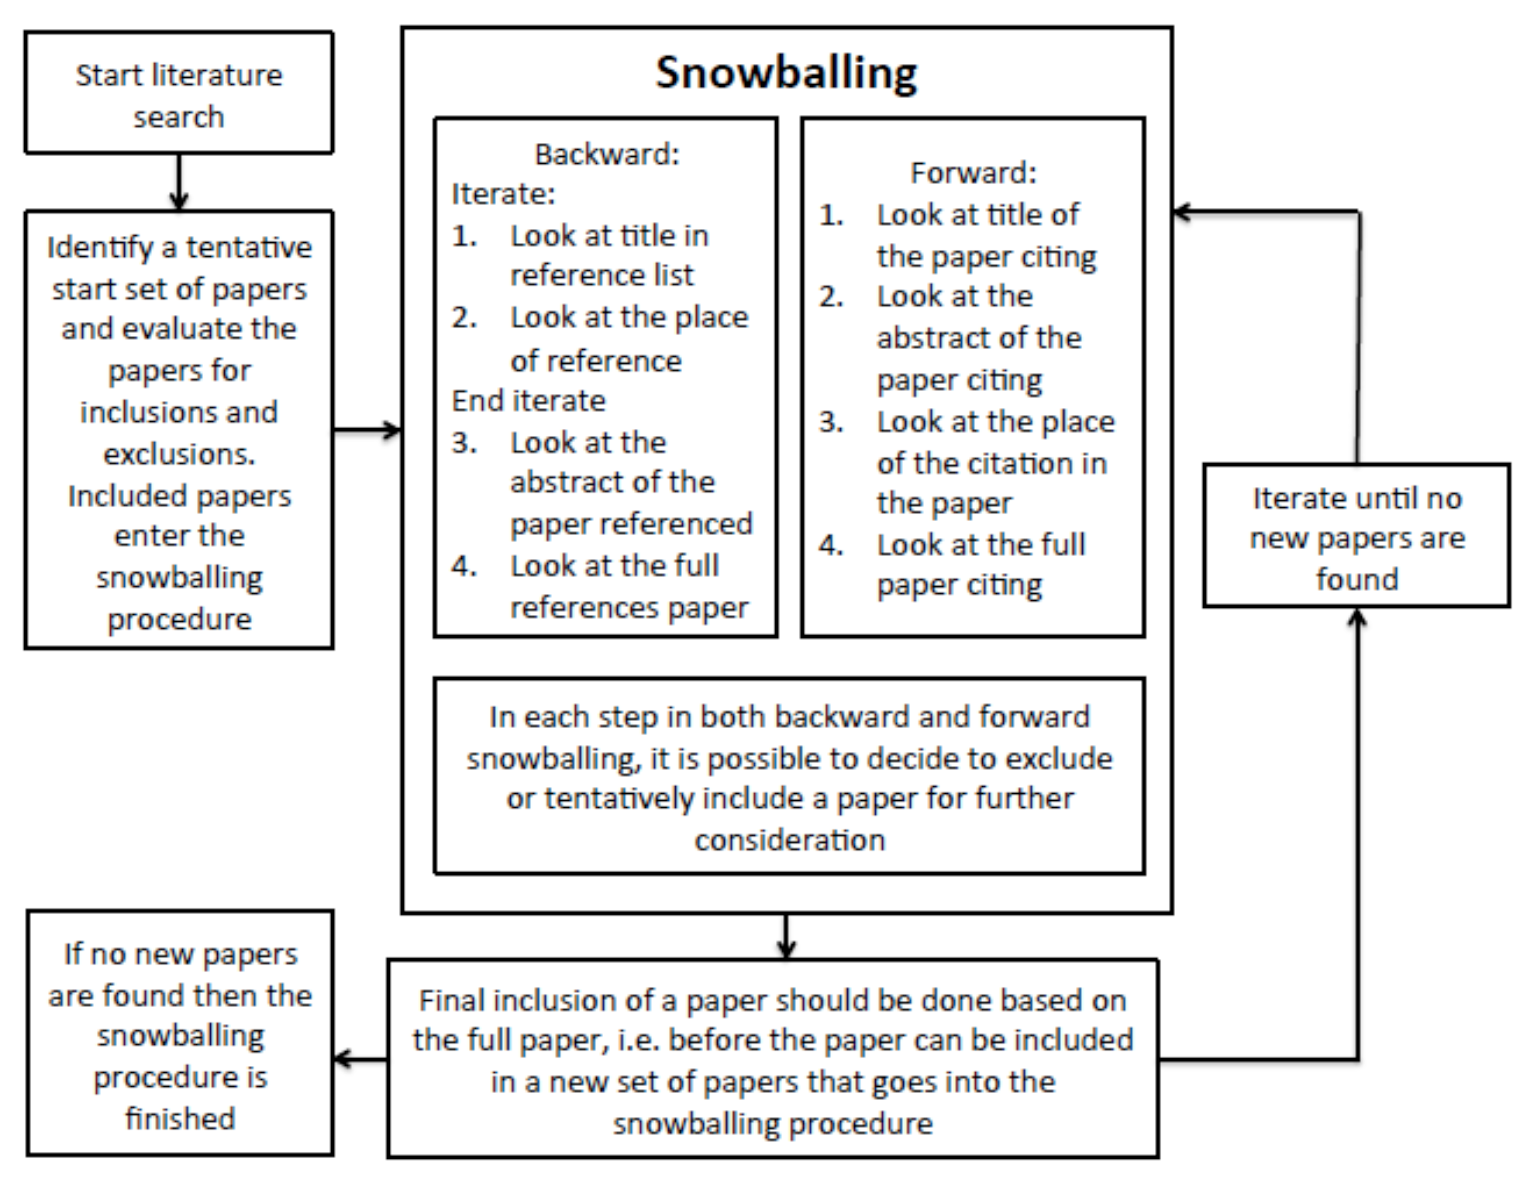
\includegraphics[width=16cm, height=12cm]{imagens/snowballing.png}
%     \legend{Fonte: \citeonline{snowballing4guidelines}.}
%     \label{figs/batepapo}  % Adicionando o label para a figura
% \end{figure}

\section{Considerações Finais}
Se necessário escreva consideracoes finais e faça o link com o que será visto no proximo capítulo

 % Desenvolvimento %
%---------------------------------------------------------------------------------------------------------
\chapter{Revisão Literária}\label{cp:revisaoliteraria}
Foi feito uma busca exploratoria utilizando a ferramenta Google Scholar  para encontrar artigos que fosse relevante ao tema e foi encontrado \cite{kratochvila2024multi} com o conteúdo desse e de similares foi gerado e refinado a string de busca.

\section{Busca Bibliográfica}\label{cp:refteory:figuras}
Foi feito a busca nas bibliotecas: arXiv e IEEExplore, nos períodos de 2021 e 2025, com a seguintes strings de busca:
   
\subsection{arXiv}
Utilizando a bibloteca python https://pypi.org/project/arxiv/
String de Busca arXiv: 
\begin{verbatim}
('(all:"floor plan" OR all:floorplan OR all:floorplans 
    OR all:"architectural layout" OR all:"building layout") ' 
'AND (all:"3D reconstruction" OR all:"3D model" 
    OR all:"layout reconstruction" OR all:"vectorization" 
    OR all:"raster-to-vector" OR all:"plan-to-3D" 
    OR all:"scene   generation" OR all:"3D scenes" OR all:Plan2Scene)'
'AND (all:"deep learning" OR all:"semantic segmentation" 
OR all:"multi-task" OR all:"multi-task learning" 
    OR all:"graph neural network" OR all:GNN 
    OR all:CNN OR all:YOLO OR all:DeepLab 
    OR all:"geometric optimization") '
'AND submittedDate:[20190101 TO 20251231] '
'ANDNOT (all:"point cloud" OR all:LiDAR OR all:LIDAR  
    OR all:SLAM OR all:mapping OR all:scan 
    OR all:BIM OR all:robot OR all:navigation 
    OR all:"scene understanding" OR all:"depth estimation")')
\end{verbatim}
\subsection{IEEExplore}
String de Busca IEEExplore:
\begin{verbatim}
("3D reconstruction" OR "3D modeling" OR "3D generation") 
AND ("floor plan" OR "architectural plan") 
AND ("deep learning" OR "semantic segmentation")
\end{verbatim}

\begin{quadro}[H]
\centering
\caption{Quantitativo das etapas de busca 
e triagem bibliográfica (2021\\-\\2025)}
\label{quadro:busca_invertido}
\begin{tabular}{|l|c|c|c|c|}
\hline
\textbf{Etapa} & \textbf{arXiv} & \textbf{IEEE Xplore}  & \textbf{Total Consolidado} \\
\hline
Total Recuperado & 56 & 14 & 70 \\
Após Título e/ou Abstract & 11 & 3 & 14 \\
Após Leitura Completa & 2 & 1 & 3 \\
\hline
Incluídos & 2 & 1 & 3 \\
\hline
\end{tabular}
\legend{Fonte: Autor}
\end{quadro}

% precisa apontar para o parágrafo da fonte? E como que escreve isso LaTeX

% Este capítulo define o protocolo de revisão utilizado para obtenção de trabalhos com propostas semelhantes as definidas nesse estudo, tal como a fundamentação teórica necessária para os conceitos apresentados no \autoref{cp:refteory}.

\section{Protocolo de Revisão}\label{cp:revisao:protocolo}

Foi usado a biblioteca python para fazer a busca no arxiv com a string de busca.

Foi usado o site do IEEE Explore para fazer a a busca com a string de busca.

Foi usando a ferramenta Rayyan para fazer a filtragem dos artigos.

\subsection{Critérios de Exclusão}
\begin{itemize}
    \item LiDAR - \textit{light detection and ranging}.
    \item Slam  - \textit{Simultaneous localization and mapping}.
    \item Point Clouds - Nuvem de pontos.    
\end{itemize}



\section{Considerações Finais}
% Protocolo de obtenção dos artigos
% Frameworks com abordagens diferentes com foco na promoção do engajamento e motivação do usuário.
Neste capítulo foram apresentados o protocolo de revisão e os trabalhos relacionados com os \nameref{cp:intro:obj} deste estudo. ....


Na busca bibliográfica \cite{kratochvila2024multi} se tornou o artigo principal de referência, ele referência os demais artigos que encontrei na busca bibliográfica, com ele pode identificar os datasets e quais são as técnicas utilizados atualmente, e se necessário fazer \textit{backtracking} para encontrar mais informações.
%--------------------------------------------------x------------------------------------------------------

 % Conclusões e Trabalhos Futuros %
%---------------------------------------------------------------------------------------------------------
\chapter{Proposta e Metodologia}\label{cp:metodologia}
Para a formulação dos procedimentos de pesquisa, retoma-se o objetivo proposto neste estudo:
Irei usar a plaforma do Google Collab para o treinamento e inferência
Irei usar o dataset CubiCasa5k
Irei usar o Pytorch para a criação do modelo
Irei usar o 
\begin{quotation}
\textit{ --  }
\end{quotation}

Este capítulo visa relatar o processo metodológico utilizado para desenvolvimento do estudo (\autoref{cp:intro:metodos}), o cronograma de tarefas (\autoref{cp:proposta:cronograma}) e os resultados que se espera obter ao fim do prazo de execução da monografia (\autoref{resultados}).

\section{Método e Procedimentos de Pesquisa}\label{cp:intro:metodos}
 ....

Com base nessas informações, do ponto de vista dos objetivos, esse estudo pode ser considerado uma pesquisa .... As etapas de desenvolvimento do projeto de pesquisa ...:

\begin{enumerate} 
\item ...

\end{enumerate}

\section{Cronograma de Pesquisa}\label{cp:proposta:cronograma}
O \autoref{cronograma} apresenta o cronograma mensal de atividades necessárias para desenvolvimento da pesquisa proposta ...

Criação de figura 

\begin{quadro}[!htb]
    \centering
    \caption{Cronograma de desenvolvimento das atividades de pesquisa.}\label{cronograma}
    \begin{tabular}{|l|c|c|c|c|}
    \hline
    & \multicolumn{4}{|c|}{2025} \\ \cline{2-5}
    \textbf{Atividades}&  Janeiro&  Fevereiro&  Março& Abril\\ \hline  
    1. Rev. Biblio.&  X&  X&  X& X \\ \hline  
    2. Map. teo. BD&  X&  X&  & \\ \hline  
    3. Exp. Elementos Design&  X&  X&  & \\ \hline  
    4. Def. Elementos &  X&  X&  & \\ \hline  
    5. Prop. Métricas&  X&  X&  & \\ \hline  
    6. Desen. do Framework&  &  X&  X& \\ \hline  
    7. Util. Framework&  X&  &  X& X\\ \hline  
    8. Escrita&  &  X&  X& X\\ \hline  
    9. Defesa&  &  &  & X\\ \hline 
    \end{tabular}

    \vspace{1cm}
    
\end{quadro}

\section{Resultados Esperados}\label{resultados}
 


%--------------------------------------------------x------------------------------------------------------

%--------------------------------------------------x-----------------------------------------------------

%--------------------------------------------------x-----------------------------------------------------


%--------------------------------------------------x-----------------------------------------------------
% ----------------------------------------------------------
% ELEMENTOS PÓS-TEXTUAIS
% ----------------------------------------------------------
%{Referencias Bibliograficas}
%---------------------------------------------------------------------------------------------------------
\bibliography{biblio.bib}
\printindex

% ---------------------------------------------------------------------
    % GLOSSÁRIO
    % --------------------------------------------------------------------- 
    % Arquivo que contém as definições que vão aparecer no glossário
    %\input{tex/glossario}
    % Comando para incluir todas as definições do arquivo glossario.tex
    %\glsaddall
    % Impressão do glossário
    %\printglossaries

    % ----------------------------------------------------------
    % Apêndices
    % ----------------------------------------------------------
    
    % ---
    % Inicia os apêndices
    % ---
   % \apendices{
    %    \chapter{References Set}
    %    \label{apendice:setinicial}
    %    \input{trabRelacionados}

   % }
    % ---
    

    % ----------------------------------------------------------
    % Anexos
    % ----------------------------------------------------------
    
    % ---
    % Inicia os anexos
    % ---
    %\anexos{
    
    
    %\begin{anexosenv}
    
        
    %\end{anexosenv}
    %}
    % ---


\end{document}